\documentclass{article}

\usepackage[a4paper, margin=1in]{geometry}
\usepackage[preprint]{neurips_2024} % Use this line for submission/drafts
\usepackage[utf8]{inputenc}
\usepackage[T1]{fontenc}
\usepackage{hyperref}
\usepackage{url}
\usepackage{booktabs}       % professional-quality tables
\usepackage{amsfonts}       % blackboard math
\usepackage{nicefrac}       % compact symbols
\usepackage{microtype}      % microtypography
\usepackage{xcolor}         % colors
\usepackage{graphicx}       % for figures
\usepackage{amsmath}        % for math
\usepackage{amssymb}        % for math symbols like \mathbb{R}
\usepackage{tikz}
\usepackage{lscape} % for landscape page
\usepackage{longtable} % for multi-page tables
\usepackage{rotating} 
\usepackage{lmodern}
\usepackage[T1]{fontenc}
\usepackage{textcomp}
\title{Self-Supervised Learning via Deep Learning-based World Models: Final Report}

\author{
    Hamza, A., \& Sanchez, A. \\
    Department of Electrical and Computer Engineering \\
    New York University Tandon School of Engineering \\
    \texttt{ah7072@nyu.edu | aas10269@nyu.edux}
}

\begin{document}
\maketitle

\begin{abstract}
 In this study, we explore the integration of Image-based Joint-Embedding Predictive Architecture (I-JEPA) with the NAVSIM Data-Driven Non-Reactive Autonomous Vehicle Simulation framework. I-JEPA, a self-supervised learning paradigm designed to model predictive abstractions without relying on generative pixel-space reconstruction, is particularly well-suited for the structured yet stochastic nature of driving environments. We leverage real-world camera sensor data extracted from the NAVSIM dataset to train the I-JEPA model, capturing the spatiotemporal dependencies inherent in dynamic road scenes. Additionally, the report reviews NAVSIM's benchmark tests performed on the trained I-JEPA model for car trajectory prediction. 
\end{abstract}

\section{Introduction}
Autonomous driving systems critically depend on robust perception modules capable of accurately interpreting complex driving environments. As the field of machine learning grows the need for machines to see the world in a more "human-like" view has been a key component in many research endeavors. 
Reliable perception enables autonomous vehicles to identify and respond appropriately to diverse road conditions, environmental changes, and dynamic obstacles, thus significantly enhancing safety, efficiency, and overall operational effectiveness. A decision-making model explored in this paper is Self-supervised learning (SSL), it has emerged as a powerful paradigm for representation learning, eliminating the need for large labeled datasets while achieving competitive performance in downstream tasks. Among SSL approaches, the \textit{Implicit Joint-Embedding Predictive Architecture} (I-JEPA) offers a novel framework that learns by predicting high-level latent representations of missing image regions, rather than reconstructing pixels or enforcing contrastive invariance. This property makes I-JEPA particularly suitable for domains requiring \textit{semantic abstraction}, such as autonomous driving that requires instant decision making in complex scenarios.

However, achieving consistently reliable perception remains challenging, primarily due to the dependence on extensive annotated datasets required by traditional supervised learning approaches. Such datasets are not only expensive and labor-intensive to produce but frequently lack sufficient diversity and variability to adequately train robust models capable of performing effectively across different scenarios and conditions. These limitations have prompted researchers and industry stakeholders alike to explore alternative approaches to perception model training.

In this research, we propose an innovative approach integrating I-JEPA with NAVSIM—a sophisticated, data-driven, non-reactive autonomous vehicle simulation and benchmarking platform designed to replicate realistic driving scenarios. Our method involves leveraging an ImageNet pre-trained I-JEPA Vision Transformer (ViT-B/16) encoder, provided by Meta AI, as a fixed or partially fine-tuned feature extractor and training it using extensive real-world imagery captured by camera sensors from the NAVSIM dataset. This dataset, rich in visual complexity and representative of diverse driving conditions, allows the model to learn nuanced and detailed representations that closely mirror real-world perception challenges. This visual backbone is combined with a lightweight MLP planning head that processes ego-vehicle status and predicts future trajectories. Due to computational resource constraints, we conduct fine-tuning and evaluation on representative subsets of the NAVSIM dataset. 

We propose experiments to evaluate the performance of this I-JEPA-based agent against baselines using NAVSIM's Predictive Driver Model Score (PDMS) and specifically assess its label efficiency by training on varying fractions of the data subset. This work explores the potential of transferring powerful, general-purpose visual representations learned via I-JEPA to the complex, sequential decision-making task of autonomous driving planning, aiming for improved data efficiency.

%By training I-JEPA on these real-world images, our approach effectively captures realistic visual variations, complexities, and intricacies inherent to actual driving environments, thereby significantly enhancing the generalization and adaptability of perception modules. NAVSIM benchmark techniques provide comprehensive tools for systematically evaluating the robustness and performance of these self-supervised representations across various critical perception tasks, including lane marking detection, obstacle classification, pedestrian recognition, and environmental understanding under diverse conditions such as varying lighting, weather, and urban complexity.

%Through rigorous experimental evaluation using NAVSIM benchmarking, we validate the efficacy of our integrated approach. Our findings demonstrate substantial improvements in the accuracy, resilience, and robustness of autonomous vehicle perception modules when employing I-JEPA-trained representations compared to traditional supervised learning methods. Notably, our approach effectively reduces the dependency on annotated data while simultaneously bridging the simulation-to-real-world performance gap.

%Ultimately, this study emphasizes the considerable potential of combining advanced self-supervised learning methodologies, such as I-JEPA, with sophisticated simulation frameworks like NAVSIM. The resulting integration represents a significant advancement towards scalable, robust, and economically viable autonomous driving systems, paving the way for more practical and widespread adoption of autonomous vehicle technologies.
\label{sec:related}

\section{Importance of Accurately Predicting a Driving Path}
\label{sec:Importance}

Self-supervised learning methods have emerged as a particularly promising alternative, offering the capability to learn informative representations from unlabeled data by leveraging intrinsic structures within the data itself. Among these, the Image-based Joint-Embedding Predictive Architecture (I-JEPA) stands out as a cutting-edge framework capable of learning robust and generalizable representations through predictive self-supervised objectives. Unlike conventional supervised approaches, I-JEPA does not depend heavily on labeled datasets, enabling more scalable, cost-effective, and flexible training strategies.

Training I-JEPA on these real-world images, our approach effectively captures realistic visual variations, complexities, and intricacies inherent to actual driving environments, thereby significantly enhancing the generalization and adaptability of perception modules. NAVSIM benchmark techniques provide comprehensive tools for systematically evaluating the robustness and performance of these self-supervised representations across various critical perception tasks, including lane marking detection, obstacle classification, pedestrian recognition, and environmental understanding under diverse conditions such as varying lighting, weather, and urban complexity.

\section{I-JEPA’s Existing Applications in Driving}

The application of self-supervised learning to autonomous driving has gained momentum, with I-JEPA being recently explored in the context of 3D object detection. A major advancement in this area is AD-L-JEPA \citep{zhu2025ad}, which extends I-JEPA to LiDAR-based representation learning. Instead of reconstructing raw point cloud data, AD-L-JEPA predicts embeddings from spatially unknown regions. It improves the quality of the data modeling. What is meant by this is that the embeddings contain relevant details about specific objects in the image that could have been hidden or not captured otherwise. 

Empirical evaluations have shown that AD-L-JEPA outperforms prior self-supervised LiDAR models such as Occupancy-MAE and ALSO, demonstrating superior transferability to 3D object detection tasks. This reinforces the idea that predictive feature-space learning is more effective than pixel-wise reconstruction for autonomous perception \citep{zhu2025ad}.

However, no direct application of I-JEPA to camera-based autonomous driving exists. The majority of prior research has focused on contrastive learning (e.g., BYOL, SimCLR, DINO) and generative approaches (MAE, Occupancy-MAE), leaving a gap in the exploration of latent-space predictive learning for end-to-end vision-based driving tasks.

\section {Overview of Theoretical Foundations}
\subsection{I-JEPA: Theoretical Foundations}

\subsubsection{Overview of Joint-Embedding Predictive Architecture (I-JEPA)}
The \textit{Implicit Joint-Embedding Predictive Architecture} (I-JEPA) \citep{assran2023self} is a self-supervised learning framework that learns by predicting high-level latent representations of missing image regions, rather than reconstructing raw pixels. Unlike traditional generative models that require pixel-wise reconstruction, I-JEPA operates in a \textit{feature space}, allowing it to learn more abstract and semantic representations. This is possible by the transformers in the architecture that makes I-JEPA which translates an incoming image into a lower dimensional space keeping the most relevant information of the image. 

I-JEPA follows a \textit{predictive modeling} approach, where the model learns to infer unseen portions of an input image using only its contextual information. This approach is inspired by human perception, where understanding is derived from partial observations rather than complete reconstructions. This characteristic makes I-JEPA particularly effective in learning transferable representations that can generalize across multiple downstream tasks, such as classification, segmentation, and object detection. Thus allowing it to work in many scenarios without depending on the pixels of an image. 

\subsubsection{Core Principles: Context and Target Encoders, Feature Space Prediction}
I-JEPA consists of three primary components:
\begin{itemize}
    \item \textbf{Context Encoder:} Processes a visible portion of the input (referred to as the \textit{context block}) and encodes it into a latent space representation(compressing the image into lower dimension but still keeping it's important features).
    \item \textbf{Target Encoder:} Independently encodes the withheld regions (\textit{target blocks}) into feature representations. Unlike contrastive learning, these target blocks are not augmented variants of the same input but rather different masked-out regions. In other words the Target Encoder takes in the same image that goes into the context encoder, and masks out certain regions of an image. It takes these masked regions and compresses it into a latent space dimension. 
    \item \textbf{Predictor Network:} A lightweight neural network that takes both the context encoding, target encoding and attempts to predict the target encoding in feature space. 
\end{itemize}

I-JEPA does not need to encode the entire input image, and only takes in a section of the image that has not been masked by the target encoder. This allows it to not have to intake numerous unlabeled data, and only a subset. Instead of directly reconstructing pixel-level details, the predictor is trained to minimize the difference between the predicted and actual target embeddings, typically using an $\ell_2$ loss function in the representation space. This design ensures that I-JEPA captures \textit{high-level semantic information} rather than low-level textures, making it more efficient for representation learning.

\subsubsection{Advantages Over Generative and Contrastive Methods}
I-JEPA differs from existing self-supervised learning approaches in several fundamental ways:

\paragraph{1. No Pixel Reconstruction (vs. Generative Models like MAE)} Masked Autoencoders (MAE) \citep{he2021masked} learn by reconstructing missing pixel values from a heavily masked image. This forces the model to focus on low-level pixel statistics rather than learning abstract, semantic concepts. In contrast, I-JEPA operates in feature space, allowing it to learn more structured and semantically meaningful representations.

\paragraph{2. No Contrastive Loss or Data Augmentations (vs. SimCLR, BYOL)} Contrastive learning methods like SimCLR \citep{chen2020simple} and BYOL \citep{grill2020bootstrap} rely on aggressive data augmentations and instance discrimination. These methods require large batch sizes and careful negative sampling to avoid collapse. I-JEPA, in contrast, does not use negative samples or augmentation-based instance discrimination. 

\paragraph{3. More Efficient and Scalable} Since I-JEPA does not require explicit contrastive negatives or complex generative decoders, it is computationally more efficient. It scales effectively with Vision Transformers (ViTs) and has been shown to perform well even with limited computational resources. 

\subsection{NAVSIM: Theoretical Foundations}
\label{sec:navsim}
\textbf{NAVSIM} \cite{dauner2024navsim} serves as a large-scale, data-driven simulation framework designed specifically for benchmarking autonomous vehicle planning agents. It utilizes real-world sensor recordings from the OpenScene dataset \cite{OpenScene2023}, which provides multimodal data including camera imagery, LiDAR point clouds, and HD map information for a single \emph{ego-vehicle}. The primary task within NAVSIM is trajectory planning: given sensor data history, current ego status, and a high-level driving command, the agent must predict the ego-vehicle's future trajectory as a sequence of $(x, y, \theta)$ poses in its local coordinate frame, typically over a 4-second horizon.

A key characteristic of NAVSIM is its \textbf{non-reactive simulation} approach for evaluation. While the ego-vehicle's predicted trajectory is simulated forward using a kinematic model and controller to check for feasibility and safety, the background traffic agents strictly follow their recorded log trajectories. This design choice ensures deterministic reproducibility and computational efficiency, allowing large-scale evaluation directly on real sensor data without requiring complex reactive agent modeling or synthetic sensor generation.

Evaluation in NAVSIM relies on simulation-based metrics aggregated into the \textbf{Predictive Driver Model Score (PDMS)} \cite{dauner2024navsim, hallgarten2023pdm}. Instead of solely relying on displacement errors relative to the human driver (which can be misleading \cite{zhairet2023rethinking}), PDMS assesses the quality of the planned trajectory by simulating its execution and measuring critical aspects like:
\begin{itemize}
    \item Safety: No-collision (NC) with other agents or static objects (with at-fault logic), Drivable Area Compliance (DAC), Time-to-Collision (TTC).
    \item Comfort: Limits on longitudinal/lateral acceleration and jerk (C).
    \item Progress: Ego Progress (EP) along the intended route compared to a reference planner.
\end{itemize}
These sub-metrics are combined into a single scalar score ($[0, 1]$), providing a holistic assessment of planning performance. The framework also supports filtering mechanisms to remove penalties if the recorded human driver also violated a specific rule (False-Positive Penalty Filtering).

For standardized training and testing, NAVSIM provides curated data splits, \texttt{navtrain} and \texttt{navtest}. These are derived from the full OpenScene dataset but filtered to enrich the proportion of challenging driving scenarios where simple heuristic policies often fail \cite{dauner2024navsim}. For our vision-based agent development, the essential inputs provided by NAVSIM for each scenario timestep include:
\begin{enumerate}
    \item The front camera image (\texttt{cam\_f0}).
    \item Past ego motion history (velocity and acceleration).
    \item A discrete driving command (e.g., left, straight, right) derived from the planned route.
\end{enumerate}

\begin{figure}[ht]
    \centering
    % Resize the whole picture to fit the line width
    \resizebox{\linewidth}{!}{% Add this line
    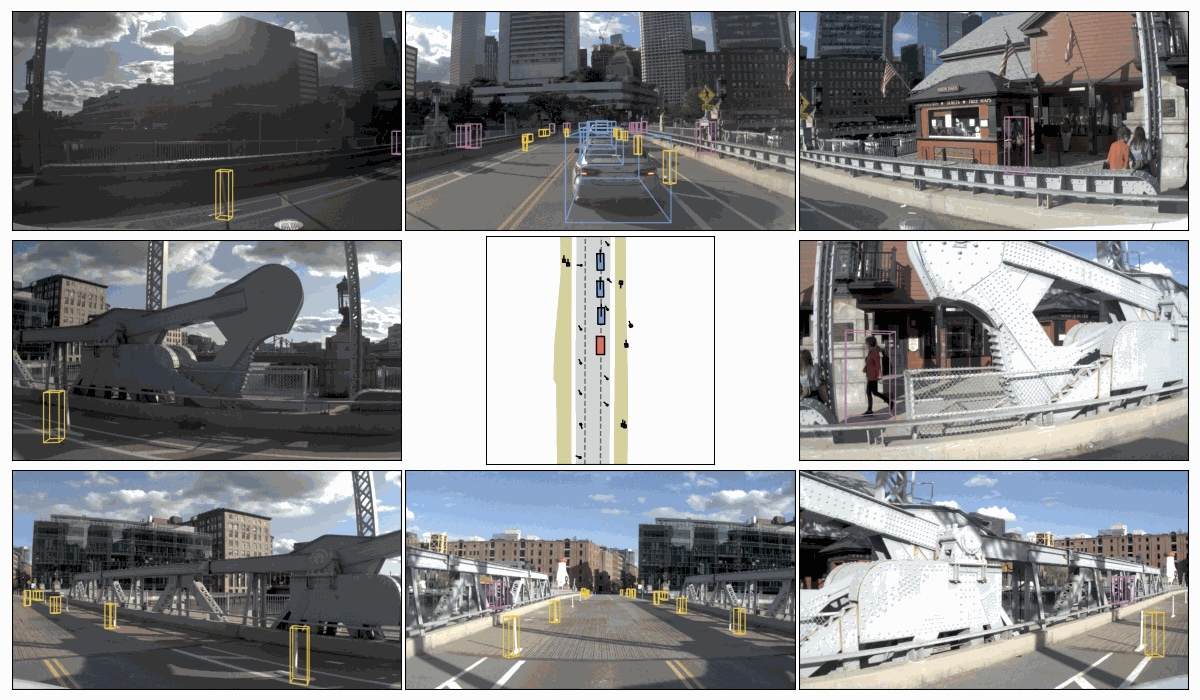
\includegraphics[width=0.8\linewidth]{images/data-sample-1.jpg}
    \hfill
    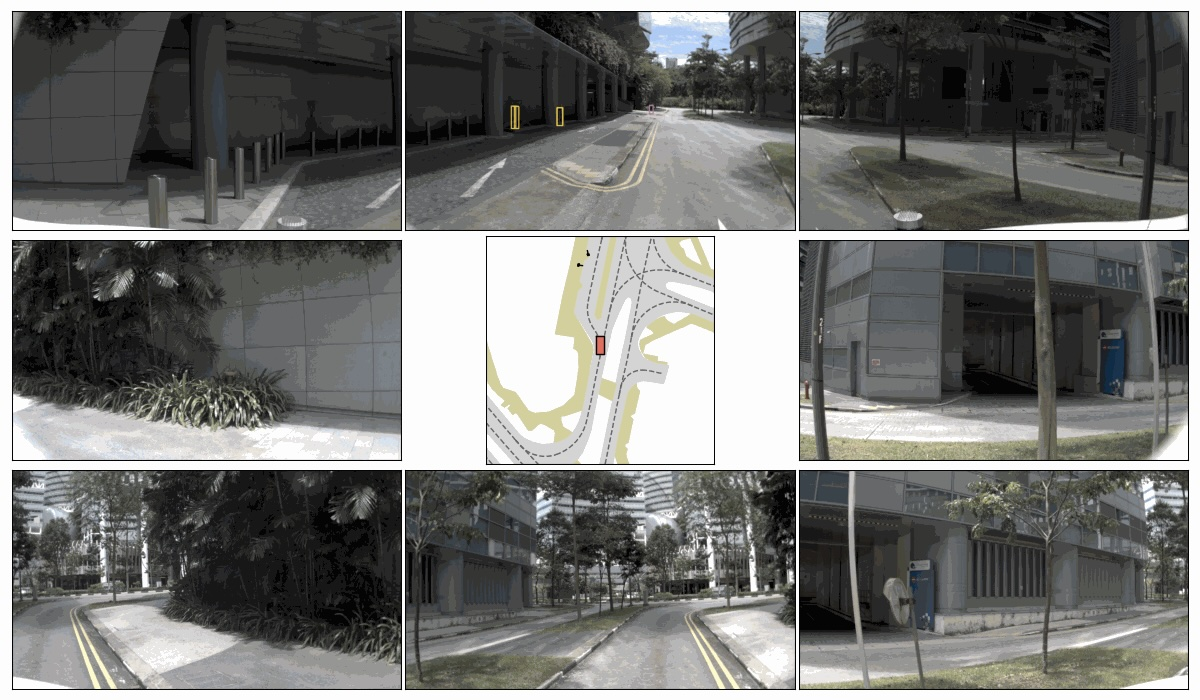
\includegraphics[width=0.8\linewidth]{images/data-sample-2.jpg}
    }
    \caption{NAVSIM frames of various cameras and sensors}
    \label{fig:navsim_scenario}
\end{figure}

While other sensor data like LiDAR is available, our approach focuses primarily on leveraging the visual input via the I-JEPA encoder as shown in Figure~\ref{fig:navsim_scenario}. 


\section{Methodology}

\subsection{Pre-trained I-JEPA Encoder}
\label{subsec:encoder}
% State the chosen approach directly and justify it.
Our approach leverages a publicly available, pre-trained I-JEPA model to serve as the visual encoder for our NAVSIM planning agent. This strategy allows us to utilize powerful, general-purpose visual features learned on large-scale datasets (ImageNet-1K) without undertaking the computationally intensive self-supervised pre-training process ourselves. We specifically adopt the official \textbf{ViT-B/16} I-JEPA checkpoint released by Meta AI \cite{assran2023ijepa}.

% Specify which parts are used and discarded.
From the complete I-JEPA architecture associated with the checkpoint, we isolate and utilize only the \textbf{context encoder} component ($f_\theta$). The target encoder ($f_{\bar{\theta}}$) and the predictor network ($g_\phi$), which are essential for the I-JEPA pre-training objective, are discarded for our downstream planning task.

% Detail the integration process: how the encoder processes NAVSIM input.
The selected ViT-B/16 context encoder has specific input requirements. To integrate it into our NAVSIM agent, the following processing pipeline is applied at each timestep the agent needs to make a prediction:
\begin{enumerate}
    % Step 1: Input Extraction - Explicitly mention the source camera.
    \item The image from the ego-vehicle's primary front camera (\texttt{cam\_f0}) is obtained from the current NAVSIM scenario data \cite{dauner2024navsim, OpenScene2023}.
    % Step 2: Preprocessing - Must match pre-training.
    \item The extracted image undergoes preprocessing to match the conditions under which the ViT-B/16 encoder was pre-trained: it is resized and center-cropped to $224 \times 224$ pixels.
    % Step 3: Normalization - Crucial for pre-trained models.
    \item Standard ImageNet normalization statistics (mean=[0.485, 0.456, 0.406], std=[0.229, 0.224, 0.225]) are applied to the pixel values.
    % Step 4: Encoder Forward Pass - The core step.
    \item The preprocessed image tensor is then passed through the loaded ViT-B/16 context encoder ($f_\theta$).
    % Step 5: Feature Extraction - Specify the exact feature used.
    \item The final visual feature representation for the planning head is obtained by extracting the output embedding corresponding to the special \texttt{[CLS]} token \cite{dosovitskiy2020vit}. For the ViT-B/16 architecture, this results in a feature vector $z_{\text{vis}} \in \mathbb{R}^{768}$.
\end{enumerate}

% Describe how the encoder's weights are handled during downstream fine-tuning.
During the subsequent fine-tuning phase on the NAVSIM trajectory prediction task (detailed in Sec.~\ref{subsec:subset}), the parameters of this pre-trained encoder are managed according to one of two strategies:
\begin{itemize}
    \item \textbf{Stage 1 (Frozen Encoder):} Initially, all parameters of the loaded ViT-B/16 encoder are frozen (i.e., their gradients are not computed or updated). Training only affects the parameters of the planning head (Sec.~\ref{subsec:head}). This stage evaluates the direct utility of the off-the-shelf ImageNet-trained I-JEPA features for the driving task.
    \item \textbf{Stage 2 (Partial Fine-tuning, Optional):} After an initial training period with the encoder frozen, we may selectively unfreeze the parameters of the final transformer block(s) and associated layer normalization layers within the ViT encoder. These layers, along with the planning head, are then trained jointly, typically employing a much smaller learning rate for the encoder parameters ($\alpha_{\text{enc}}$) compared to the head ($\alpha_{\text{head}}$) (e.g., $\alpha_{\text{enc}} = \alpha_{\text{head}} / 10$). This allows the higher-level features of the encoder to adapt slightly to the specific visual characteristics of the NAVSIM environment while aiming to preserve the robust representations learned during pre-training.
\end{itemize}

% \subsection{Planning Head}
% \label{subsec:head}
% We employ a simple Multi-Layer Perceptron (MLP) as the planning head. This head takes the concatenated visual features and ego status information as input and predicts the future trajectory.
% \begin{itemize}
%     \item \textbf{Input Features:} The input to the MLP is the concatenation of the visual feature $z_{\text{vis}} \in \mathbb{R}^{768}$ (from the I-JEPA encoder's \texttt{[CLS]} token) and the current ego status features $z_{\text{ego}} \in \mathbb{R}^{7}$. The ego status features consist of 2D velocity, 2D acceleration, and a 3-dimensional one-hot encoding of the driving command (left, right, straight), resulting in a combined input dimension of $768 + 7 = 775$.
%     \item \textbf{Architecture:} The MLP consists of two hidden layers, each with 256 neurons and ReLU activation functions.
%     \item \textbf{Output:} The final linear layer maps the 256-dimensional hidden representation to the flattened trajectory parameters. For a 4-second horizon sampled at 0.5-second intervals ($N_{\text{poses}} = 8$), the output dimension is $N_{\text{poses}} \times 3 = 8 \times 3 = 24$. This output is then reshaped into the trajectory format $[N_{\text{poses}}, 3]$, where each row represents $(x, y, \theta)$ in the local ego-vehicle coordinate frame at future timesteps $\{0.5, 1.0, \dots, 4.0\}\,\text{s}$.
%     \item \textbf{Training Loss:} The planning head (and optionally the unfrozen encoder layers) is trained using an $L_1$ loss between the predicted trajectory and the ground-truth future trajectory recorded by the human driver in the NAVSIM logs.
% \end{itemize}

\subsection{Planning Head}
\label{subsec:head}
The planning head serves as the crucial component that maps the rich features extracted by the visual encoder and the current vehicle state into a concrete future trajectory plan. For this initial investigation, we employ a relatively simple \textbf{Multi-Layer Perceptron (MLP)} architecture for this head.

% Justification for choosing MLP
The choice of an MLP is deliberate, driven by several factors:
\begin{itemize}
    \item \textbf{Simplicity and Efficiency:} MLPs are straightforward to implement, computationally efficient to train and run, and provide a solid baseline for regression tasks.
    \item \textbf{Focus on Features:} By using a simple head, we aim to primarily evaluate the quality and utility of the semantic features ($z_{\text{vis}}$) derived from the pre-trained I-JEPA encoder. A more complex head (e.g., a Transformer decoder) might achieve higher performance but could also obscure whether improvements stem from the head's architecture or the input features themselves.
    \item \textbf{Baseline Establishment:} It establishes a performance benchmark. If strong results can be achieved even with this simple head, it strongly suggests the high quality of the I-JEPA features for this task. Future work could then explore more complex head architectures.
\end{itemize}

% Detailed Structure Description
The specific structure of our MLP planning head is as follows:
\begin{itemize}
    \item \textbf{Input Features:} The input layer receives the concatenated feature vector, combining the visual embedding $z_{\text{vis}} \in \mathbb{R}^{768}$ (from the I-JEPA encoder's \texttt{[CLS]} token, Sec.~\ref{subsec:encoder}) and the current ego status features $z_{\text{ego}} \in \mathbb{R}^{7}$ (2D velocity, 2D acceleration, and a 3-dimensional one-hot encoding for the driving command: left, right, or straight). This results in a combined input vector of dimension $768 + 7 = 775$.
    \item \textbf{Hidden Layers:} The MLP incorporates two hidden layers.
        \begin{itemize}
            \item The first hidden layer performs a linear transformation from the 775-dimensional input to 256 neurons, followed by a Rectified Linear Unit (ReLU) activation function. ReLU is chosen for its computational efficiency and ability to introduce non-linearity, allowing the network to model complex relationships.
            \item The second hidden layer applies another linear transformation from 256 neurons to 256 neurons, again followed by a ReLU activation.
        \end{itemize}
    \item \textbf{Output Layer:} A final linear layer maps the 256-dimensional representation from the last hidden layer to the required output dimension for the trajectory. For the standard NAVSIM 4-second planning horizon sampled at 0.5-second intervals ($N_{\text{poses}} = 8$), the output consists of 8 poses, each with $(x, y, \theta)$ coordinates. Therefore, the output layer has $N_{\text{poses}} \times 3 = 8 \times 3 = 24$ neurons. This layer uses \textit{no activation function}, as is standard for regression tasks where the output values are unbounded (or bounded by subsequent processing/interpretation rather than the activation itself).
    \item \textbf{Output Reshaping:} The flattened 24-dimensional output vector is then reshaped into the standard trajectory format $[N_{\text{poses}}, 3]$ (i.e., $[8, 3]$), where each row represents the predicted $(x, y, \theta)$ pose in the local ego-vehicle coordinate frame at future timesteps $\{0.5, 1.0, \dots, 4.0\}\,\text{s}$.
\end{itemize}

% Justification for L1 Loss
\paragraph{Training Loss:}
The parameters of the planning head (and potentially the unfrozen encoder layers during Stage 2 fine-tuning) are optimized by minimizing the \textbf{L1 loss} (Mean Absolute Error) between the predicted trajectory and the ground-truth future trajectory recorded by the human driver in the NAVSIM logs.

L1 loss was chosen over alternatives like L2 loss (Mean Squared Error) for several reasons relevant to trajectory regression:
\begin{itemize}
    \item \textbf{Robustness to Outliers:} L1 loss is generally less sensitive to large errors or outliers in the ground-truth data compared to L2 loss, which squares the difference. Human driving trajectories can occasionally contain sharp, atypical maneuvers which might unduly influence a model trained with L2 loss.
    \item \textbf{Direct Interpretation:} L1 loss directly minimizes the average absolute error in predicted coordinates and heading, providing an interpretable penalty on the magnitude of deviation from the ground truth.
    \item \textbf{Common Practice:} L1 loss is frequently employed for trajectory prediction tasks in autonomous driving literature, facilitating comparisons and aligning with established practices.
\end{itemize}

\subsection{Fine-tuning on NAVSIM Subsets}
\label{subsec:subset}
The standard training configuration within the NAVSIM framework utilizes the \texttt{navtrain} split \cite{dauner2024navsim}. This split is itself a curated filter applied to the large OpenScene \texttt{trainval} dataset logs, specifically selecting over 100,000 challenging driving scenarios where simple heuristic policies often fail. While NAVSIM offers optimized sensor data downloads for \texttt{navtrain} (approx. 445GB), processing even this curated split for numerous experiments can be demanding under the NYU HPC quota limitations and time constraints.

Therefore, to ensure feasible training times and resource usage, our fine-tuning experiments are conducted on a further \textbf{randomly selected subset} derived from the official \texttt{navtrain} split. We define a fixed subset fraction, specifically \textbf{10\%} (corresponding to \(\approx\) 10,300 scenarios), sampled once based on scenario tokens. This fixed training subset is used consistently across all experiments, including the training of baseline models (Sec.~\ref{sec:experiments}) and the label efficiency analysis, ensuring fair comparisons.

From this selected training subset, a small portion (e.g., 10\%) is held out to form a distinct \textbf{validation subset}. This validation set is used exclusively for monitoring training progress (e.g., validation loss) and potentially for early stopping, preventing overfitting to the training subset. The NAVSIM \texttt{Dataset} class and data loading scripts are configured to load only the scenario tokens corresponding to our defined training and validation subsets.

The fine-tuning process will make use the AdamW optimizer \cite{loshchilov2017decoupled} with default hyperparameters, except for the learning rate. We train for a maximum of 50 epochs, using the validation subset loss for potential early stopping. A base learning rate, $\alpha_{\text{head}}$, is applied to the parameters of the planning head (Sec.~\ref{subsec:head}). 

For the Stage 2 partial fine-tuning (Sec.~\ref{subsec:encoder}), the learning rate for the unfrozen encoder parameters, $\alpha_{\text{enc}}$, is reduced, $\alpha_{\text{enc}} = \alpha_{\text{head}} / 10$. To gauge the robustness of our findings concerning the chosen subset and training stochasticity, key experiments may be repeated using multiple random seeds for the initial subset sampling and model weight initialization.

% \begin{figure}[h]
%     \centering
%     % Placeholder: Replace with your actual plot later
%     \includegraphics[width=0.6\linewidth]{placeholder_label_efficiency.png}
%     \caption{Planned evaluation: PDM-Score vs. fraction of labeled training subset. We expect the I-JEPA agent (blue) to outperform the Ego Status MLP baseline (orange), especially in the low-data regime.}
%     \label{fig:efficiency_plan}
% \end{figure}

\section{Experiments}
% Experiments goes here
\subsection{NAVSIM Dataset:}
The  chosen OpenScene \cite{Open2023op}, a redistribution of nuPlan \cite{Nap2024to}, the largest annotated public driving dataset. OpenScene
includes 120 hours of driving at a reduced frequency of 2Hz typically considered by end-to-end
planning algorithms, resulting in a 90\% reduction of data storage requirements compared to nuPlan
from over 20 TB to 2 TB. Our agent input, based on OpenScene, comprises of one front view camera, with a resolution of 1920 × 1080 pixels. The input
includes the current time-step and optionally 3 past frames, totaling 1.5s at 2Hz.\cite{dauner2024navsim}

\subsection{PDM Score}
The benchmarks provided by NAVSIM to evaluate our agent are the following:
\footnotesize%%%%%%%%%%%  smaller font size %%%%%%%%
%\begin{landscape}
\renewcommand{\arraystretch}{1.5} % more space between rows
\begin{longtable}{|p{2.2cm}|p{4.0cm}|p{7.2cm}|}
\hline
\textbf{Metric} & \textbf{Formula} & \textbf{Description} \\
\hline
PDM (Path Deviation Metric) & 
$\displaystyle \text{PDM} = \frac{1}{T} \sum_{t=1}^T \| \hat{\mathbf{p}}_t - \mathbf{p}_t \|_2$ &
Measures the mean Euclidean distance between the predicted and ground-truth trajectories. Lower is better. \\
\hline
NC (No-At-Fault Collisions) &
$\displaystyle \text{NC} = \frac{1}{N} \sum_{i=1}^N \mathbb{1}\left( \text{collision\_at\_fault}(i) = 0 \right)$ &
Fraction of scenarios where the ego-agent avoids collisions it would be considered at fault for. \\
\hline
DAC (Drivable Area Compliance) &
$\displaystyle \text{DAC} = \frac{1}{T} \sum_{t=1}^T \mathbb{1}\left( \hat{\mathbf{p}}_t \in \mathcal{D} \right)$ &
Percentage of predicted trajectory points remaining within drivable areas. \\
\hline
DDC (Driving Direction Compliance) &
$\displaystyle \text{DDC} = \frac{1}{T} \sum_{t=1}^T \mathbb{1}\left( \cos \theta_t \geq \delta \right)$ &
Evaluates if predicted heading maintains alignment with lane heading directions. \\
\hline
TLC (Traffic Light Compliance) &
$\displaystyle \text{TLC} = \frac{1}{T_{\text{crossings}}} \sum_{k=1}^{T_{\text{crossings}}} \mathbb{1}\left( \text{light\_state}(k) \in \{\text{Green}, \text{Yellow}\} \right)$ &
Assesses compliance with traffic light signals when crossing intersections. \\
\hline
EP (Ego Process Stability) &
$\displaystyle \text{EP} = \frac{1}{T} \sum_{t=1}^T \mathbb{1}\left( \| \text{Jerk}_t \|_2 \leq J_{\text{max}} \right)$ &
Evaluates stability and physical plausibility of ego-vehicle motions, penalizing high jerks. \\
\hline
TTC (Time-to-Collision within Bound) &
$\displaystyle \text{TTC}_{i,j}(t) = \frac{ \| \mathbf{p}_i(t) - \mathbf{p}_j(t) \|_2 }{ \| \mathbf{v}_i(t) - \mathbf{v}_j(t) \|_2 }$ &
Ensures predicted trajectories maintain a minimum safe Time-to-Collision (TTC) with surrounding agents. \\
\hline
LK (Lane Keeping) &
$\displaystyle \text{LK} = \frac{1}{T} \sum_{t=1}^T \mathbb{1}\left( \hat{\mathbf{p}}_t \in \mathcal{L} \right)$ &
Measures the extent to which predicted trajectories stay within designated lane boundaries. \\
\hline
C (History Comfort) &
$\displaystyle \text{C} = \frac{1}{T_h} \sum_{t=1}^{T_h} \| \text{Jerk}_t \|_2$ &
Quantifies smoothness of historical trajectory by computing mean jerk values. Lower is better. \\
\hline
TFEC (Two-Frame Extended Comfort) &
$\displaystyle \text{TFEC} = \frac{1}{T-1} \sum_{t=1}^{T-1} \| \hat{\mathbf{a}}_{t+1} - \hat{\mathbf{a}}_{t} \|_2$ &
Assesses smoothness and comfort across consecutive predicted frames by analyzing changes in acceleration. \\
\hline
\end{longtable}
\subsection{Overview of I-JEPA Agent Model in NAVSIM Environment}
Our I-JEPA model created follows NAVSIM's 'AbstractAgent' as a parent structure. The following classes and functions were included in our agent. 

\subsubsection{Class FirstBatchDebugger}
\begin{itemize}
    \item \textbf{on\textunderscore train\textunderscore batch\textunderscore start:} This function trains and prints the first 3 relative and normalized predictions of the first batch of the dataset. 
\end{itemize}
\subsubsection{Class BatchInspector}
\begin{itemize}
    \item \textbf{on\textunderscore train\textunderscore batch\textunderscore end:} Function prints the shape or the way the features and targets being trained look like every 100 batches. 
\end{itemize}
\subsubsection{Class CameraImageFeatureBuilder}
\begin{itemize}
    \item \textbf{get\textunderscore unique\textunderscore name:} print name 'front\textunderscore camera\textunderscore image'
    \item \textbf{compute\textunderscore features:} Takes front sensor camera 0 image and converts it to a tensor array.
\end{itemize}
\subsubsection{Class EgoFeatureBuilder}
\begin{itemize}
    \item \textbf{get\textunderscore unique\textunderscore name:} 
    \item \textbf{compute\textunderscore features:} 
\end{itemize}
\subsubsection{Class TrajectoryTargetBuilderGT}
\begin{itemize}
    \item \textbf{get\textunderscore unique\textunderscore name:} prints name 'ego\textunderscore features'
    \item \textbf{compute\textunderscore targets:} 
\end{itemize}
\subsubsection{Class IJEPAPlanningAgent}
\begin{itemize}
    \item \textbf{name:} 
    \item \textbf{initialize:} 
    \item \textbf{get\textunderscore sensor\textunderscore config:} 
    \item \textbf{get\textunderscore feature\textunderscore builders:} 
    \item \textbf{get\textunderscore target\textunderscore builders:} 
    \item \textbf{forward:}
    \item \textbf{compute\textunderscore loss:}
    \item \textbf{get\textunderscore optimizers:}  
    \item \textbf{get\textunderscore training\textunderscore callbacks:}
\end{itemize}

\subsection{Results and Discussion}
\paragraph{Results and Discussion}
% Experiments goes here

\paragraph{Conclusion}
% conclusion goes here

\bibliographystyle{unsrt}
\bibliography{references}

\end{document} HI
ALI HANMZA- ALI HANZ HAMZA HAM HAM HAMBURGER
